\chapter{More on tidal formalisms}
\label{appendix:tideFormalisms}
\section{Response}
\citet{Godin:1991vx} describes the response method as a cross spectral analysis.  The analysis aims to characterise an LTI model in frequency-space on the basis of paired input and output timeseries.
Whereas harmonic methods evolved well before the availability of machine computers, the response method relies on computational signal processing with discretely sampled and finite length time series.
A response analysis aims to empirically characterise the LTI as a complex-valued transfer function on the basis of output coherence with the inputs. 
\begin{quotation}
The goal of any response formalism is to accurately predict the ocean tides by an optimum smooth function, realising that the ocean tides are mostly, although not completely, predictable.
\end{quotation}
The outcome of a response analysis is not a single admittance curve, but rather a small number of distinct curves; typically the semi-diurnal, diurnal and long-period tides associated with degree-2 spherical harmonics $(n,m)=(2,2),(2,1),(2,0)$.\\
Smoothness of $Z(\omega)$ within each distinct tidal band is a core principle behind methods for determining admittances.  
\begin{align}
    \label{E:response}
    g(\Delta t) + \dots &\Rightarrow & \fbox{empirical admittance curves $Z$} &\Rightarrow & \mbox{$\eta(\Delta t)$}  %\nonumber
\end{align}
Where $g(\Delta t)$ is a discretely sampled input signal, nominally the equilibrium tide.   Figure \ref{fig:response} schematically illustrates the process.
Once determined the admittance curves can map a tidal input to a tide prediction.
%% admittance
%\begin{equation}
%\label{E:Z}
%\eta(t) = \sum_{n=2}^{3}\sum_{m=0}^{n}\sum_{k} H_{nmk} \text{Re} \left[ %Z_{nm}(\omega)^*e^{-i(t\theta_{nmk})} \right] 
%\end{equation}
The presence of incoherent noise in the observational timeseries means that determining each admittance curve $Z$ is not simply the matter of division in frequency-space.


In order to distinguish coherent signal from incoherent noise, Munk and Cartwright introduce the \emph{convolution formalism}. The convolution technique exploited the band-concentration of tidal spectra into semi-diurnal, diurnal and long period species and the associated assumption of \emph{smooth} admittances within each of these bands.  A complex-valued admittance $Z(i\omega)$ is fitted separately to each band-limited species via a convolution operation in time-space. 
Inversion of a smooth admittance function from tidal records can be classed as a discrete-time/continuous-frequency operation \citep{Percival:1998tw}.

There is however, no unique manner in which to formulate the problem.  Munk and Cartwright formulated the convolution with a discrete time-kernal of `lag weights' to be applied to a finite record of regularly sampled data. % as in equation \ref{E:lags}.   
This is equivalent to modelling the smooth admittance in each band as a finite (and periodic in frequency) Fourier series.   Although no physical meaning is attributed to the periodicity of the admittance in frequency, in the context of band-concentrated tidal energy, this allows for a compact convolution kernal consisting of only a very small number of `lags`.   The design of this convolution kernal requires a choice of the number of lags $s$ and lag interval $\Delta T$.  Equivalently, this design sets the period and number of Fourier components used to model the admittance function.  For instance, in an application of this convolution formalism to altimetry data, \citet{Smith:1997ut} choose $\Delta T=2$ days and $s=3$.   Note that what at face value may seem a rather long lag of 2 days relates to the \emph{bandwidth} of the tidal species rather than a timescale of tidal variation.

From this perspective, a tidal signal is written as a weighted sum of past (and possibly future) values of the driving input function. 
Tidal analysis subsequently consists of empirically determining a series of weight values  via a least-squares minimisation on an observational timeseries.
The resultant complex weights form a time-space kernal representation of the frequency-space admittance $Z(\omega)$   In frequency-space, the minimisation problem amounts to fitting the Fourier series to model $Z(\omega)$.
%\begin{align}
%\label{E:lags}
%\eta_{tidal}(t) &= \sum_{m=0}^{2}\sum_{s=0}^{S} w_{nm}(s)c_{nm}(t-s\Delta T)\\
%              n &= 2   \nonumber
%\end{align}

The introduction of response methods in the 1960's was not motivated by a user-driven need to improve tide predictions.  It could rather been seen as a move to review the well-embedded conventions of harmonic analysis in the contemporary language of timeseries analysis and ``make explicit what the harmonic method does anyway''\citep[pp 540]{Munk:1966ts}.  In contrast to the dynamic blindness of conventional harmonic analysis, the response perspective facilitated explicit treatment of drivers other than the \ATGP{}.

Nonlinear effects are especially significant in coastal locations.   By definition, such shallow-water tides cannot be represented by a LTI model with only $\eta_{eq}$ as an input.  The response method can incorporate nonlinearity as an additional explicit input.    For instance,  in a 2-stage process, a preliminary linear analysis determines admittances for `equivalent deep water port' which are subsequently used to produce new input timeseries of paired and tripled products \citep[pp 122]{Pugh:1996uz}.
%------------------
\begin{figure}[!hbt] \centering
    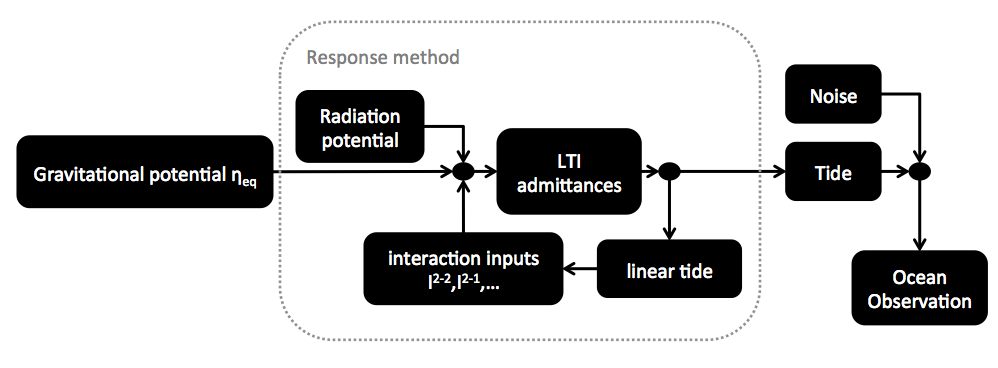
\includegraphics[width=\figwidthBig]{figures/diagrams/response_analysis_flowchart.png}
    \caption{Response method tidal schematic.}
    {Nonlinear and non-gravitational inputs are explicitly formed and the analysis process consists of empirically fitting smooth admittance curves.}
\label{fig:response}
\end{figure}
%------------------
Perhaps even more illustrative of the way in which a response analysis conceptualises tides is the formulation of the `radiational potential'.   This is an additional harmonic forcing series formulated to more explicitly account for the influence of atmospheric tides and other periodic solar effects on ocean observations. So-named due to the abstract connection with diurnal solar radiative fluxes, the radiational potential concept is rather ad hoc in comparison to developments of the \ATGP{}.  
The radiational input provided a more satisfactory formulation of observed harmonic ocean signals, S1 and S2, with amplitudes disproportionate to terms in the \ATGP{}.
From a sea level forecasting perspective, the response approach could be said to have modernised the formulation and increased the role of physical considerations, but in doing so hasn't ultimately translated to adding value for routine use in operational centres.


%\subsection{Variants}
Fitting a Fourier series via the convolution formalism to find each smooth admittance is not the only viable implementation of the response concept.  For instance a Green's function formulation is described by \citet{Webb:1974ke} and polynomial models are evaluated by \citet{Desai:1995je}. More influential though is the orthotide approach to fitting Fourier series admittances, discussed below.


% harmonics == admitance
Consistent with this equivalence, it is common within the literature to refer to harmonic constants \emph{as} admittances.   A harmonic constant is seen as a sample from the admittance curve at an exact frequency. For instance \citet{Smith:1997ut} provides the simple conversion to sample $Z(\omega_{nmk})$ and scale by the \ATGP{} amplitude $H_{nmk}$.
Furthermore, harmonic constants remain the lingua franca of ocean tide discussions. Regardless of the detail behind any particular method, results are almost universally transformed into conventional amplitude and phase values for intercomparisons.


% inference and smooth
Regardless of the method used for analysis, an expectation that admittance curves $Z(\omega)$ should not contain discontinuities or sharp changes (the `credo of smoothness') has been evoked to enhance the spectral content upon the \emph{synthesis} of a tidal timeseries.  Following an analysis performed to determine admittances at a relatively small number of frequencies, $Z{\omega}$ is interpolated or extrapolated in frequency-space to infer additional spectral information.   The design of such an inference process can treat frequencies on a case-by-case basis distinguishing between component admittance curves (for instance \citet[pp 268]{Fu:2001ub}).

\section{Orthotide}% orthotide
A possible weakness of the original convolution formalism relates to the non-orthogonality of the harmonically decomposed $c_{nm}(t)$ over finite records.  That is, unlike a Fourier series, inner products between component sinusoids comprising the tidal input are not necessarily zero.   Thus the weighting values that are determined with the response analysis are dependant on details of each particular analysis, such as the number of other components included.  Subsequently these weights cannot be assigned any independent meaning and are not amenable to communication.  
In recognising that this lack of translatable meaning is something of a step backwards from conventional tidal parameters, \citet{Groves:1975ky} introduced the \underline{orthotide formalism}.

Orthotides are orthogonalised transformations of the harmonically decomposed tidal input timeseries.
%\begin{align}
%c_{nm}(t) =  &\sum_{k} H_{nmk} e^{-i(\omega_{nmk} + \beta_{nml})}  \Rightarrow %\sum_{l}^L \overline{\zeta}_{nml}(t)     \nonumber \\
%             &\mbox{where} \langle \overline{\zeta}_p \overline{\zeta}_q \rangle  = %\delta_{pq}  \mbox{over $-\infty < t < \infty$}             \nonumber
%\end{align}
A tidal timeseries is then represented as a linear sum of these orthotide functions with so-called `orthoweights'. In essence this is no different to Munk and Cartwrights convolution, but involves an improved time-space formulation.  
The resulting orthoweights have the attractive property of not being dependant on the number of components involved in any particular analysis, and subsequently could be said to share some of the characteristics of conventional tidal constants.
%\begin{equation}
%\label{E:orthosum}
%\eta_{tide}(t) = \sum_{n=2}^3 \sum_{m=0}^n \sum_{l}^L \overline{\zeta}_{nml}(t)
%\end{equation}

Regardless of the formulation of time-space convolution, the determination of weights is equivalent to fitting smooth admittance curves - which is the ultimate goal of the response method.  The fitting process is a minimisation problem with degrees of freedom equal to the number of free parameters to be determined.    The length of timeseries and signal to noise ratio are balanced against the assumption of smoothness in $Z$.
\begin{quotation}   
The use of orthotides may provide some benefits to the empirical determination of ocean tide models from a short duration of observations, but is otherwise unnecessary. \dots  polynomial and orthotide, and therefore convolution, approaches to modelling the smooth admittance function provided similar results as long as they are defined by an identical number of parameters.\citep{Desai:2006wo}
\end{quotation}
